%!TEX root = synthese.tex
\newpage
\section{Introduction}

L’objectif du projet Qualité Test était de réaliser, en respectant les exigences qualité demandées, un jeu multi-joueurs. Le but du jeu est d’être le premier pirate à découvrir un trésor sur le plateau de jeu. L’ensemble du jeu sera développé en java et des tests devaient être effectués tout au long de l’implémentation du jeu. 

\section{Diagramme de classe}

Nous avons séparé le projet en trois packages : \\

\begin{itemize}
\item Le package \textbf{commande} qui regroupe les classes qui gèrent la commande;
\item Le package \textbf{model} qui représente la logique du serveur. Ce package regroupe la gestion du jeu en général (déplacements des personnages, création des nouveaux pirates, initialisation d’une partie, etc.);
\item Le package \textbf{network}  se consacre à la connexion et la communication entre le serveur et les clients.\\ 
\end{itemize}

Nous avons implémenté deux design-pattern pour la réalisation de ce projet : \\

\begin{itemize}
\item Le \textbf{Singleton}. Le singleton est l’île. C’est à dire qu’il existe une unique instance de l’objet Island qui est partagée auprès de tous les clients;
\item L’\textbf{Observer}. Si il y a un changement sur l’île, tous les pirates sont notifiés. 
\end{itemize}


\begin{figure}[!ht]
	\centering
	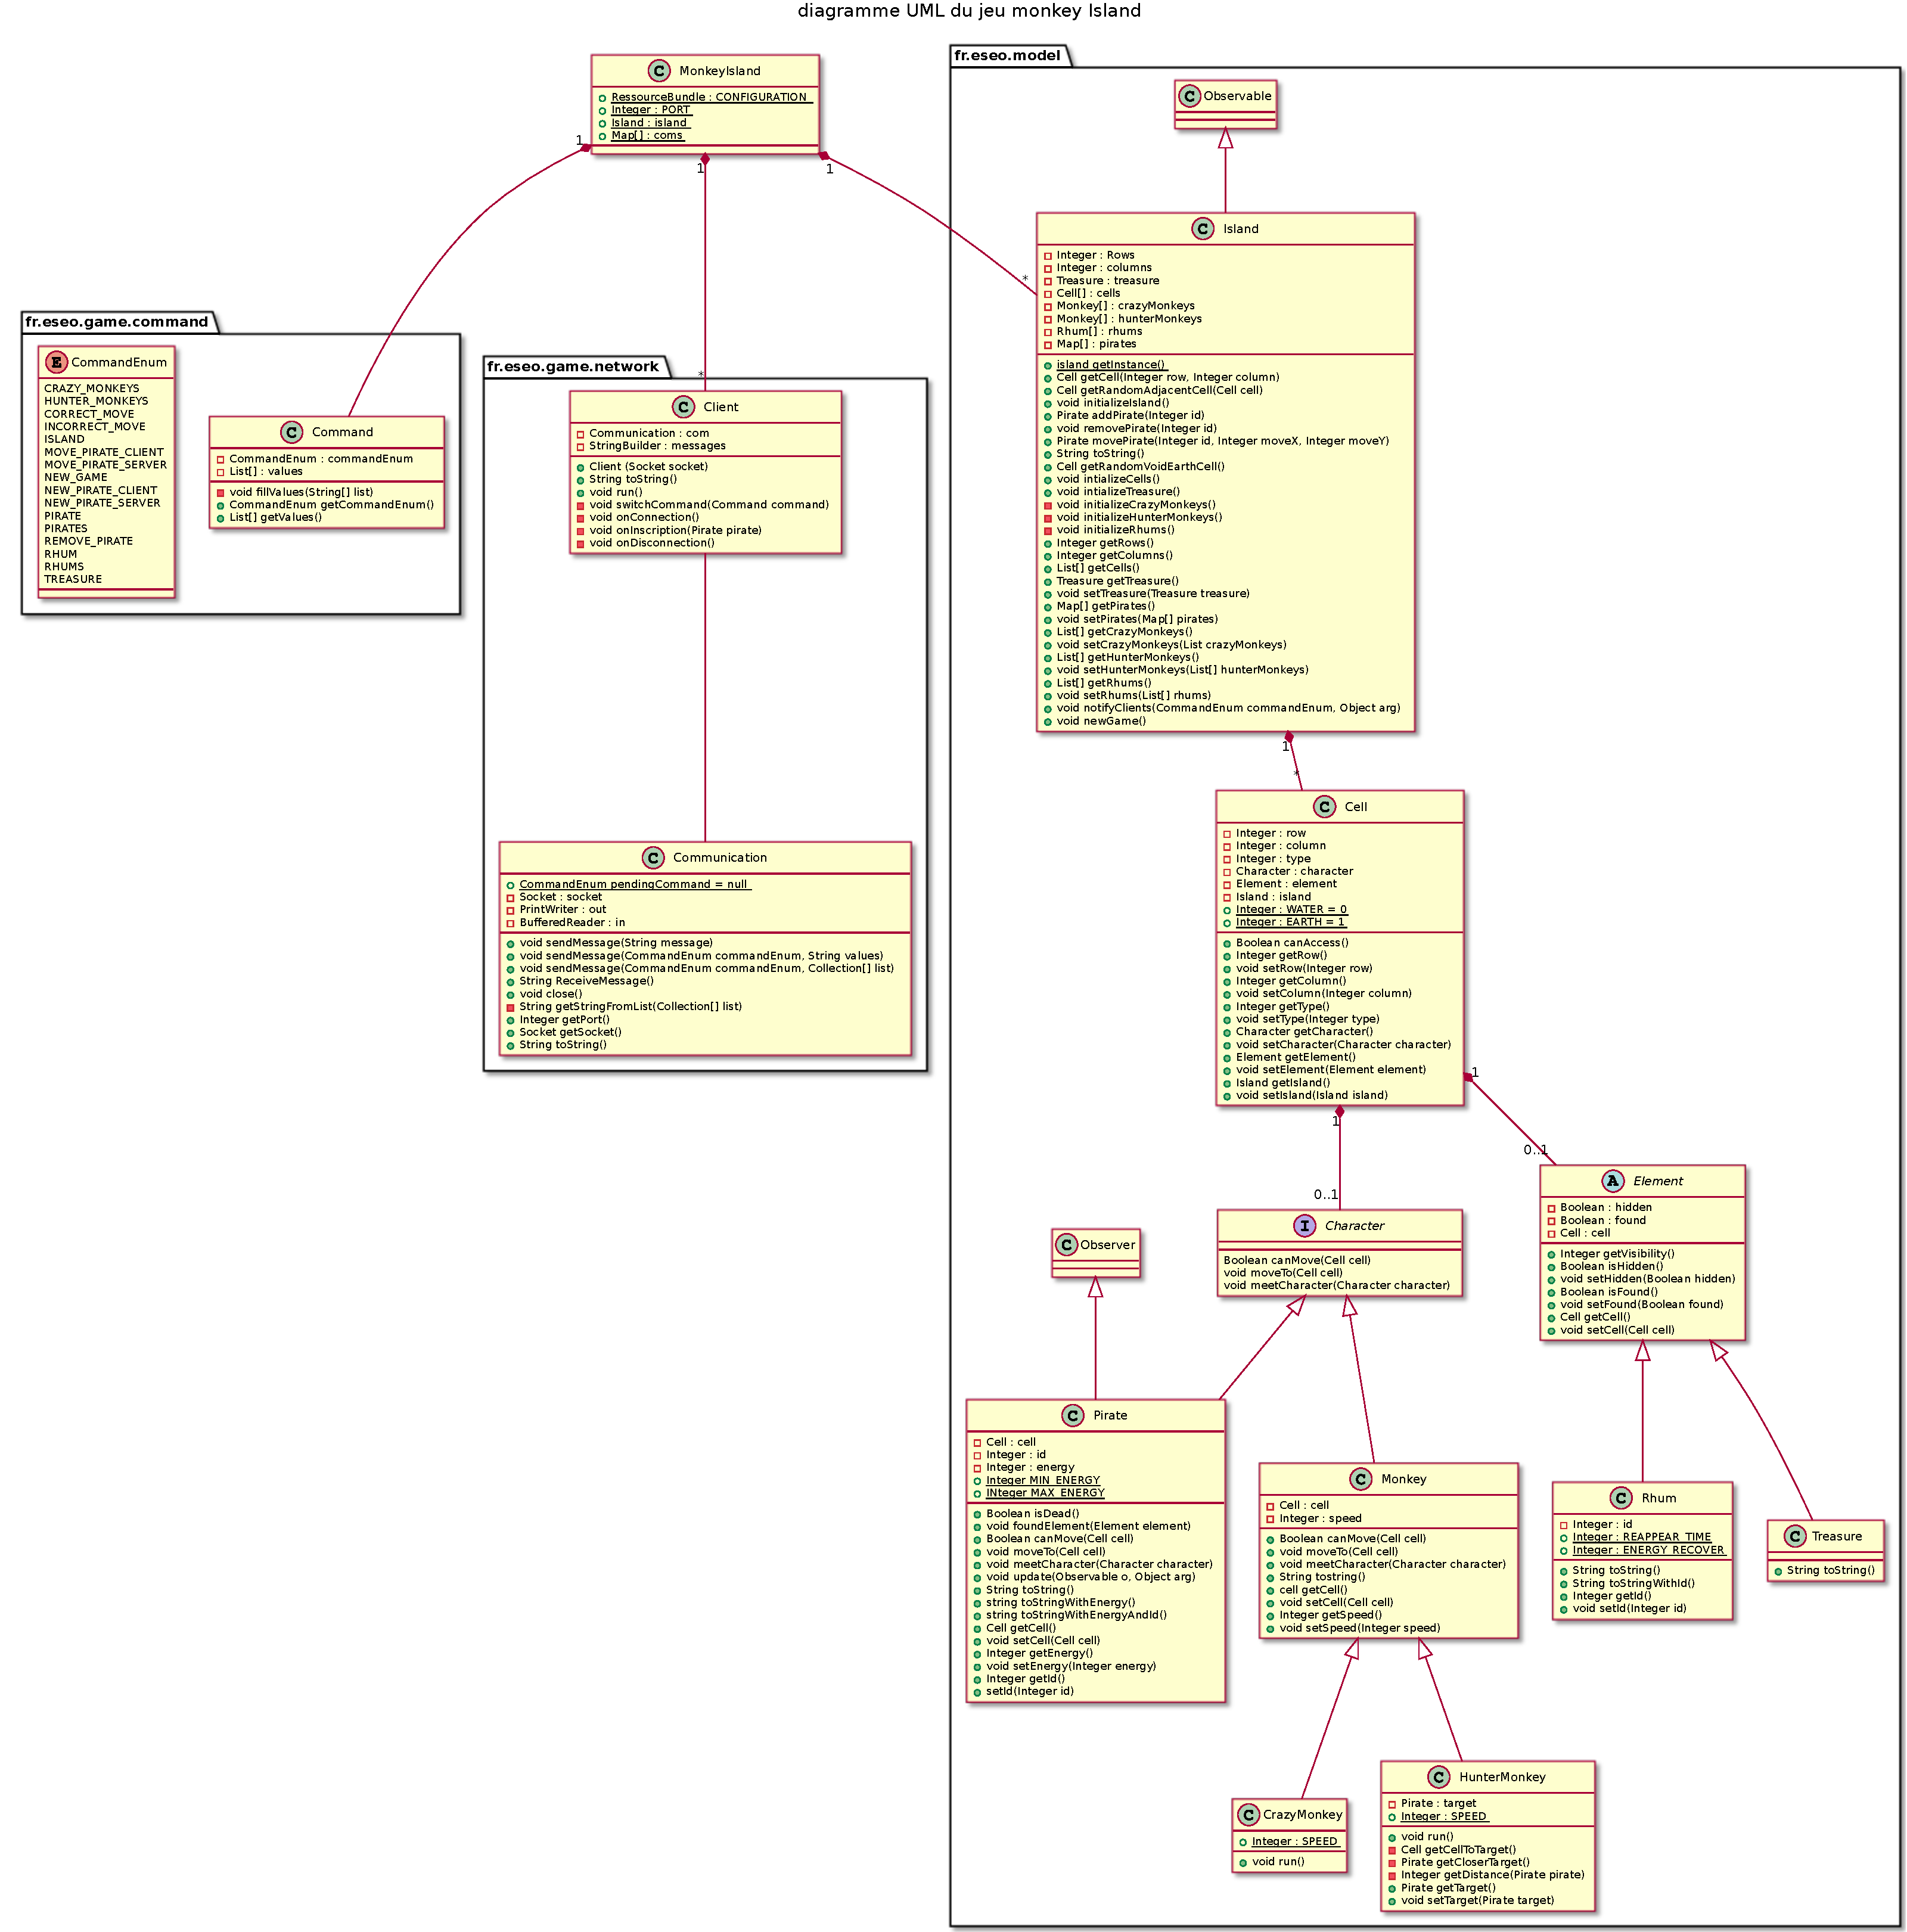
\includegraphics[width=\textwidth]{images/plantuml.pdf}
\end{figure}


\clearpage
\section{Incrément 1}
Le premier incrément devait rassembler les fonctionnalités suivantes:
\begin{itemize}
\item Le déplacement des singes erratiques,
\item Le gestion des pirates (déplacement et décès),
\item La gestion du trésor,
\item La communication client-serveur.\\
\end{itemize}

Nous avons testé avec Junit toutes les méthodes publiques des classes \emph{Monkey}, \emph{Pirate}, \emph{Treasure} et \emph{Island} et \emph{Cell}.\\

Afin de déplacer les singes, nous avons utilisé un \emph{thread} pour chaque singe. La méthode \emph{run} est appelée toute les secondes (vitesse du singe) grâce à la classe Java : \emph{ScheduledExecutorService} et la méthode  \emph{scheduleAtFixedRate}.

\begin{lstlisting}
ScheduledExecutorService execCrazy = Executors.
	newSingleThreadScheduledExecutor();
    for (Monkey monkey : island.getCrazyMonkeys()) {
    	execCrazy.scheduleAtFixedRate(monkey, 
    		0, monkey.getSpeed(), TimeUnit.SECONDS);
    }
\end{lstlisting}

Nous avons testé le déplacement des singes erratiques dans toutes les directions (équiprobabilité), le déplacement du pirate dans toutes les directions, la rencontre des différents personnages et des éléments. Enfin, la communication a été testée avec JMeter.

\section{Incrément 2}
Le deuxième incrément devait rassembler les fonctionnalités suivantes:\\

\begin{itemize}
\item La gestion du fichier de configuration,
\item La gestion de l'énergie de chaque pirate,
\item La gestion des bouteilles de rhum,
\item La gestion des parties.\\
\end{itemize}

La gestion du fichier de configuration a été effectuée grâce à la classe Java : \emph{RessourceBundle}. Cette classe permet le chargement d'un fichier au format \emph{properties} (clé=valeur). Cet objet est stocké dans la classe \emph{MonkeyIsland}.

\begin{lstlisting}
public static final RessourceBundle CONFIGURATION = 
	RessourceBundle.getBundle("Configuration");
\end{lstlisting}

\section{Incrément 3}

Le troisième incrément devait rassembler les fonctionnalités suivantes:\\

\begin{itemize}
\item La gestion des singes chasseurs.\\
\end{itemize}

Pour les singes chasseurs, nous avons implémenté un algorithme qui détermine la cible(un pirate) pour chaque singe chasseur. Pour définir la cible la plus proche, nous calculons la distance entre le singe chasseur et les pirates présents sur le plateau. La cible d'un chasseur est donc définie comme étant le pirate qui se trouve le plus proche (la distance la plus petite).\\

Une fois la cible choisie, le singe se déplace dans la direction du pirate en incrémentant ou décrémentant la position x ou y du singe.

